\section{Kommunikation}

\todo{Överväger att lägga figur \ref{kommunikation-oversikt} i Systemet och protokollen under varje enhet.}

\begin{figure}[h!]
	\centering
	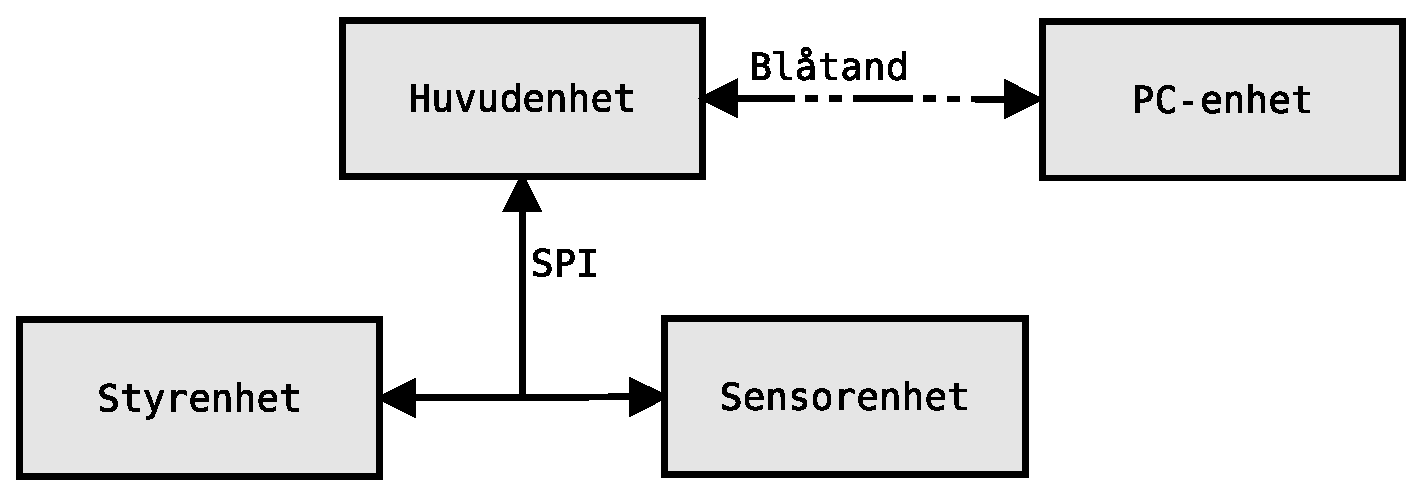
\includegraphics[scale=0.4]{grafik/kommunikation-oversikt}
	\caption{Översikt systemets kommunikationskanaler} \label{kommunikation-oversikt}
\end{figure}

Figur \ref{kommunikation-oversikt} ger en översikt av vilka moduler som kommunicerar med varandra och på vilket sätt detta sker. Styrenheten och Sensorenheten använder samma SPI-buss fast med olika Slave Select-pinnar.

\subsection{PC-enhet $\longleftrightarrow$ Huvudenhet}

PC-enheten och Huvudenheten kommunicerar över Blåtand.
\todo{Hur set det här protokollet ut i verkligheten?}

\subsection{Huvudenhet $\longleftrightarrow$ Styrenhet}

Huvudenheten kommunicerar med Styrenheten över SPI. Storleken på en instruktion är antingen fyra eller sju bytes lång. För att förebygga synkroniseringsproblem skickas först två startbytes bestående av hexadecimalt $0xff$ följt av längden på instruktionen (startbytesen och längdbyten räknas ej med). Därefter följer instruktionsbyten som består av två delar. De fyra högsta bitarna anger vilken instruktion som ska utföras enligt tabell \ref{protokoll:pc-motor-tabell}, och de fyra lägsta vilket servo eller motorpar instruktionen rör enligt tabell \ref{protokoll:pc-motor-adress-tabell}. I fallet att instruktionen är \textit{Sätt register A till D} krävs dessutom två databytes.

Då ett motorpar adresseras anger den minsta biten i den första databyten vilken riktning motorparet skall röra sig. $0$ anger framåt, $1$ bakåt \todo{Stämmer?}. Den andra databyten anger vilken fart vi vill att motorerna skall röra sig i. Notera att motorerna sätts med kommandot $Sätt register A till D$.

De servon vi arbetar med har en upplösning på 10 bitar både för position och hastighet. Vi måste alltså ha två databytes när vi vill ändra någon egenskap hos dessa. De två minsta bitarna i den första databyten är de två högsta bitarna och därefter följer den andra databyten.

\todo{Tabell för att illustrera bitar hit och dit?}

\subsection{Instruktionslista}

\begin{table}[h!]
	\centering
	\begin{tabularx}{\textwidth}{| l | l | X |}
		\hline
		\textbf{Instruktion} & \textbf{Argument} & \textbf{Beskrivning} \\\hline
		{0000} & {} & {Stoppa samtliga servon och motorer \todo{Behöver implementeras}} \\\hline
		{0001} & {A, D} & {Sätt register A till D} \\\hline
		{0010} & {A} & {Utför givna kommandon för A} \\\hline
		{0011} & {A, D} & {Sätt servohastighet för A till D} \\\hline
		{0100} & {A} & {Returnera Status för A \todo{Implementera?}} \\\hline
	\end{tabularx}
	\caption{Kommandon från huvudenhet till styrenhet \todo{Stämmer tabellen?}} \label{protokoll:pc-motor-tabell}
\end{table}

\begin{table}[h!]
	\centering
	\begin{tabularx}{\textwidth}{| l | X |}
		\hline
		\textbf{Adress} & \textbf{Beskrivning} \\\hline
		{0000} & {Höger hjulpar} \\\hline
		{0001} & {Vänster hjulpar} \\\hline
		{0010} & {Arm axel 1} \\\hline
		{0100} & {Arm axel 2} \\\hline
		{0110} & {Arm axel 3} \\\hline
		{1000} & {Arm axel 4} \\\hline
		{1011} & {Arm axel 5 (\textit{gripklo})} \\\hline
		{1100} & {Samtliga motorer} \\\hline
		{1101} & {Samtliga servon} \\\hline
		{1111} & {Samtliga motorer och servon} \\\hline
	\end{tabularx}
	\caption{Adresser för adressering till styrenhet} \label{protokoll:pc-motor-adress-tabell}
\end{table}

\subsection{Huvudenhet $\longleftrightarrow$ Sensorenhet}

Huvudenheten kommunicerar med Sensorenheten över SPI. Protokollet mellan dessa moduler är väldigt primitivt då det endast finns en instruktion, returnera sensordata för begärd sensor. Instruktionen anges av de 4 högsta bitarna av instruktionsbyten enligt tabell \ref{protokoll:huvud-sensor}. Huvudenhetens begäran är då bara på en enda databyte och Sensorenheten svarar med de 8 högsta bitarna för den efterfrågade sensorn. Vilken sensor som enheten returnerar data för anges av de 4 minsta bitarna i instruktionsbyten enligt tabell \ref{protokoll:huvud-sensor-adress}.

\subsection{Instruktionslista}

\begin{table}[h!]
	\centering
	\begin{tabularx}{\textwidth}{| l | l | X |}
		\hline
		\textbf{Instruktion} & \textbf{Argument} & \textbf{Beskrivning} \\\hline
		{0000} & {A} & {Returnera sensordata för A} \\\hline
	\end{tabularx}
	\caption{Instruktion från huvudenhet till sensorenhet} \label{protokoll:huvud-sensor}
\end{table}

\begin{table}[h!]
	\centering
	\begin{tabularx}{\textwidth}{| l | X |}
		\hline
		\textbf{Adress} & \textbf{Beskrivning} \\\hline
		{0000} & {Linjesensor 1} \\\hline
		{0001} & {Linjesensor 2} \\\hline
		{0010} & {Linjesensor 3} \\\hline
		{0011} & {Linjesensor 4} \\\hline
		{0100} & {Linjesensor 5} \\\hline
		{0101} & {Linjesensor 6} \\\hline
		{0110} & {Linjesensor 7} \\\hline
		{0111} & {Linjesensor 8} \\\hline
		{1000} & {Linjesensor 9} \\\hline
		{1001} & {Linjesensor 10} \\\hline
		{1010} & {Linjesensor 11} \\\hline
		{1011} & {Avståndssensor Höger} \\\hline
		{1100} & {Avståndssensor Vänster} \\\hline
	\end{tabularx}
	\caption{Adresser för instruktioner till sensorenhet} \label{protokoll:huvud-sensor-adress}
\end{table}
